\section{比热}\label{sec:3-3}

1 克水温度升高 1 ℃吸收的热量是 1 卡。
那么,1 克别的物质温度升高 1 ℃吸收的热量是不是 1 卡呢?
我们用实验来研究这个问题。

\begin{figure}[htbp]
    \centering
    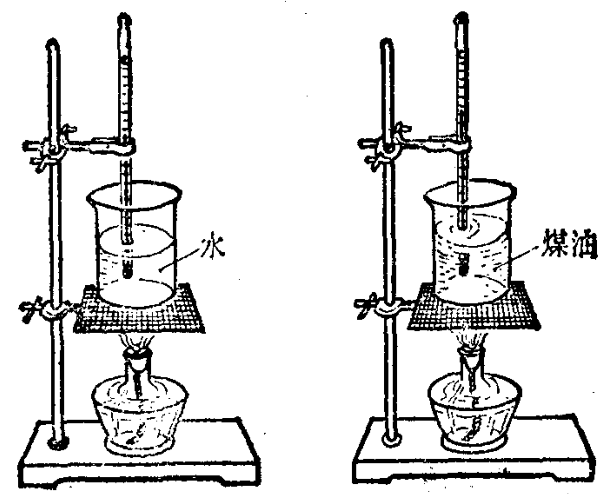
\includegraphics[width=0.5\textwidth]{../pic/czwl2-ch3-1}
    \caption{}\label{fig:3-1}
\end{figure}

拿两个同样的烧杯,分别装上质量和温度都相同的水和煤油。
用两个同样的酒精灯给它们加热。
从温度计可以看到,煤油的温度升高得比水快(图 \ref{fig:3-1})。
要使水升高的温度跟煤油的相同,就得给水加热较长的时间。
这表明,质量相等的水和煤油,升高相同的温度,吸收的热量不相等,
水吸收的热量多,煤油吸收的热量少。

换用其他物质来做这样的实验,也可以得到同样的结果。
可见,\CJKunderwave{质量相等的不同物质升高相同的温度,吸收的热量不相等}。

为了比较各种物质的这种性质上的不同,在物理学中引入了比热容这个物理量。

\textbf{单位质量的某种物质,温度升高 1 ℃吸收的热量,叫做这种物质的比热容}。
比热容通常简称为\textbf{比热}。

实验证明,单位质量的某种物质,温度降低 1 ℃放出的热量,
跟温度升高 1 ℃吸收热量相等,即等于它的比热。

如果质量的单位用克,热量的单位用卡,比热的单位就是 卡/(克·℃), 读做“卡每克摄氏度”。
如果质量单位用千克,热量单位用千卡,比热的单位就是 千卡/(千克·℃),读做“千卡每千克摄氏度”。

从下表可以看出,每种物质都有自己的比热,比热是物质的特性之一。

\begin{table}[H]
    \centering
    \caption*{几种物质的比热值[ \, 卡/(克·℃) \, 或 \, 千卡/(千克·℃) \,]}
    \begin{tblr}{
        colspec={|lc|lc|lc|lc|},
        columns={colsep+=0.5em},
    }
        \hline
        水 & 1.00 & 冰 & 0.50 & 铝 & 0.21 & 铜 & 0.093 \\
        酒精 & 0.58 & 蓖麻油 & 0.43 & 干泥土 & 0.20 & 水银 & 0.033 \\
        煤油 & 0.51 & 砂石 & 0.22 & 铁、钢 & 0.11 & 铅 & 0.031 \\
        \hline
    \end{tblr}
\end{table}

从表中可以知道,水的比热比较大。
水的这种特性,对于气温变化有显著的影响。
水和泥土、砂石相比,在同样受热或冷却的情况下,水的温度变化比泥土、砂石的慢。
这就使沿海地区的气温变化不象内陆地区的气温变化那样显著。

水的比热比较大这一特性,在农业生产中也很有用。
在培育秧苗的时候,为了保护秧苗夜间不致受冻,傍晚时向秧田里多灌一些水,
这样夜间秧田的温度不致降低太多,秧苗就不致冻坏。
第二天早晨再把田的水放出一些,以便在阳光照射下,秧田的温度可以高些,有利于秧苗的生长。

